\documentclass[10pt,a4paper]{article}
\usepackage{fontspec}
\setmainfont{Arial}
\usepackage[spanish,es-noshorthands]{babel}
\usepackage[a4paper,margin=2cm]{geometry}
\usepackage{amsmath,amssymb}
\usepackage{graphicx}
\usepackage{booktabs}
\usepackage{array}
\newcolumntype{L}[1]{>{\raggedright\arraybackslash}p{#1}}
\usepackage{tikz}
\usetikzlibrary{arrows.meta,positioning,calc,fit,backgrounds}
\usepackage{xcolor}
\usepackage{enumitem}
\usepackage{caption}
\usepackage{float}
\usepackage[hidelinks]{hyperref}
\graphicspath{{figuras_avances/}}
\captionsetup{font=small,labelfont=bf}
\setlength{\parskip}{0.5em}
\setlength{\parindent}{0pt}
\definecolor{tinta2}{HTML}{5C5C58}
\definecolor{fondo}{HTML}{F3F2EE}
\definecolor{acento}{HTML}{2A78D6}

\newcommand{\bh}{\hat\beta}
\newenvironment{preguntas}{\par\medskip\noindent{\bfseries Preguntas posibles}\par\smallskip\begin{description}[leftmargin=0pt,itemsep=0.6em,font=\normalfont\itshape]}{\end{description}}
\newcommand{\pr}[1]{\item[#1]\mbox{}\\}

\tikzset{
  bloque/.style={draw, rounded corners=2pt, minimum height=9mm, minimum width=18mm, align=center, font=\small, fill=white},
  suma/.style={draw, circle, inner sep=0pt, minimum size=5mm, font=\small},
  flecha/.style={-{Stealth[length=2.2mm]}, semithick},
  etiq/.style={font=\footnotesize, text=tinta2},
}

\title{Actuador con recorte, x0 entrenable y referencia black-box\\[2mm]\large Explicación de los resultados y preguntas posibles}
\date{}
\author{}

\begin{document}
\maketitle
\vspace{-12mm}

Este documento acompaña a la presentación de avances. Sigue el mismo orden, agrega lo que en las diapositivas queda implícito y, al final de cada sección, reúne preguntas que puede hacer quien escucha, con su respuesta. La sección 2 explica cómo se conecta el controlador con cada modelo, que la presentación no muestra.

Salvo aclaración, cada valor es la media de tres semillas. El NRMSE es el de los 13 escenarios de test que interpolan, en \%. El error de $\bh$ es el error relativo medio de los diez parámetros de Wilson-Cowan, en \%. $\sigma$ es el desvío del ruido de medición, con dos niveles, 0,01 y 0,05.

\section{Plantas, modelos y métricas}

\textbf{Simulador.} Es el sistema que genera los datos y que, en lazo cerrado, ocupa el lugar de la planta real. Es Wilson-Cowan con una perturbación que el modelo reducido no tiene. Con $S(u) = 1/(1+e^{-u})$,
\begin{align*}
\tau_i \dot I &= -I + S\big(a_i (w_{IE}E - w_{II}I + Q_{ef} - \theta_i)\big) - k_i,\\
\tau_e \dot E &= -E + S\big(a_e (w_{EE}E - w_{EI}I + P_{ef} - \theta_e)\big) - k_e .
\end{align*}
En la planta con actuador, el comando pasa por un filtro de primer orden y un recorte,
\[
\tau\,\dot P_f = P - P_f, \qquad P_{ef} = \min\!\big(3, \max(-3, P_f)\big), \qquad \tau = 1\ \text{ms},
\]
y lo mismo para $Q$. Antes del recorte se usaba $P_{ef} = 3\tanh(P_f/3)$. La otra planta es la refractaria, que multiplica cada sigmoidea por $(1 - r x)$ con $r = 0{,}10$.

\textbf{Modelos.} Todos tienen el backbone de Wilson-Cowan $f_{WC}(x, P, Q; \bh)$ con los diez parámetros entrenables, salvo la black-box.

\begin{center}
\small
\begin{tabular}{@{}lll@{}}
\toprule
modelo & campo vectorial & qué agrega al backbone \\
\midrule
white-box & $f_{WC}(x, u_k; \bh)$ & nada \\
agnóstica & $f_{WC} + g(I, E)$ & red del estado \\
historia con comando actual & $f_{WC} + g(I, E, u_k, \dots, u_{k-9})$ & red con 5 ms del comando \\
historia sin comando actual & $f_{WC} + g(I, E, u_{k-1}, \dots, u_{k-10})$ & red con 5 ms, sin el comando actual \\
filtro 8 canales & $f_{WC} + g(I, E, W u_{k:k-39})$ & 20 ms del comando por un FIR de 8 canales \\
estado de filtro & $f_{WC}(x, \hat P_{ef}; \bh)$ & $\hat\tau\dot{\hat P} = P - \hat P$, $\hat P_{ef}$ recortado en $\pm 1/\hat\alpha$ \\
black-box & $g(I, E, P, Q)$ & sin backbone \\
\bottomrule
\end{tabular}
\end{center}

$u_k$ es el comando $(P, Q)$ en la muestra $k$, con 0,5~ms entre muestras. El estado de filtro es la forma exacta de la perturbación del actuador. Para la refractaria, la forma exacta es el backbone con el factor $(1 - \hat r x)$.

\textbf{Métricas.} El NRMSE mide la reproducción en lazo abierto de estímulos que el modelo no vio. El error de $\bh$ mide cuánto se alejan los parámetros identificados de los verdaderos. El R² contra el término faltante mide cuánto de la perturbación quedó representado en la corrección. En lazo cerrado se usan el RMSE de seguimiento y la distancia al lazo con el simulador (sección 7).

\section{Cómo se conecta el controlador con cada modelo}

\subsection{La ley de control}

El controlador es el IMC del paper de referencia, con los parámetros nominales de Wilson-Cowan, que son los del simulador sin la perturbación. En este trabajo no se modifica. Tiene tres etapas.

\begin{enumerate}[leftmargin=*,itemsep=0.3em]
\item \textbf{Un PI por población.} Con $Z$ la integral del error,
\[
U_I = 10\,(r_I - I) + 5\,Z_I, \qquad U_E = 5\,(r_E - E) + 5\,Z_E, \qquad \dot Z = r - x .
\]
$U$ es la derivada que el controlador quiere imponer, en la forma $\tau_i \dot I = -I + U_I$.
\item \textbf{Inversión de la sigmoidea.} Para que la sigmoidea entregue $U_I + k_i$, su argumento tiene que valer
\[
u_q = \theta_i - \frac{1}{a_i}\ln\!\left(\frac{1}{U_I + k_i} - 1\right),
\]
y lo mismo para $u_p$. $U$ se acota antes al dominio donde la inversa existe.
\item \textbf{Cancelación del acoplamiento.} El comando resta la parte del argumento que aportan las propias poblaciones,
\[
Q = u_q - (w_{IE}E - w_{II}I), \qquad P = u_p - (w_{EE}E - w_{EI}I).
\]
\end{enumerate}

Si la planta fuera exactamente Wilson-Cowan con los parámetros nominales, el lazo quedaría $\tau_i \dot I = -I + U_I$, lineal, y el PI lo llevaría a la referencia. Es una linealización por realimentación. El controlador invierte su propio modelo interno de la planta.

\begin{figure}[H]
\centering
\begin{tikzpicture}[node distance=7mm and 9mm]
  \node[suma] (s) {};
  \node[left=8mm of s, etiq] (r) {$r_I, r_E$};
  \node[bloque, right=of s] (pi) {PI\\$U = K_p e + K_i Z$};
  \node[bloque, right=of pi] (inv) {$S^{-1}$\\(sigmoidea inversa)};
  \node[bloque, right=of inv] (des) {desacople\\$-(w E - w I)$};
  \node[bloque, right=13mm of des, minimum width=24mm, fill=fondo] (pl) {planta\\simulador o modelo};
  \node[right=10mm of pl, etiq] (y) {$I, E$};
  \draw[flecha] (r) -- (s);
  \draw[flecha] (s) -- node[above, etiq]{$e$} (pi);
  \draw[flecha] (pi) -- node[above, etiq]{$U$} (inv);
  \draw[flecha] (inv) -- node[above, etiq]{$u$} (des);
  \draw[flecha] (des) -- node[above, etiq]{$P, Q$} (pl);
  \draw[flecha] (pl) -- (y);
  \coordinate (b) at ($(pl.east)+(5mm,0)$);
  \draw[flecha] (b) -- ++(0,-14mm) -| node[pos=0.95, left, etiq]{$-$} (s);
  \draw[flecha] ($(b)+(0,-14mm)$) -| (des.south);
  \begin{scope}[on background layer]
    \node[draw=acento, dashed, rounded corners, fit=(pi)(inv)(des), inner sep=3mm, label={[etiq]above:controlador IMC, parámetros nominales, sin cambios}] {};
  \end{scope}
\end{tikzpicture}
\caption{Lazo cerrado del paper. El bloque de planta es el simulador o, en la prueba de cada modelo, el modelo identificado. El controlador usa $I$ y $E$ medidos para el error y para el desacople.}
\label{fig:lazo}
\end{figure}

\subsection{Qué cambia con cada modelo en este trabajo}

En este trabajo el modelo identificado reemplaza a la planta, y el controlador queda igual. Lo que se invierte en cada paso es siempre el Wilson-Cowan nominal del controlador, nunca el modelo identificado. La pregunta que responde la prueba es si el lazo que se forma con el modelo se parece al que se forma con el simulador. Si se parece, el modelo sirve para diseñar y probar el controlador en simulación.

\begin{figure}[H]
\centering
\begin{tikzpicture}[node distance=5mm and 8mm]
  \node[etiq] (u) {$P, Q$};
  \node[bloque, right=8mm of u, minimum width=28mm] (mem) {memoria del comando\\(según el modelo)};
  \node[bloque, right=of mem, minimum width=22mm] (red) {red $g$};
  \node[bloque, below=8mm of red, minimum width=22mm] (bb) {backbone\\$f_{WC}(x, \cdot\,; \bh)$};
  \node[suma, right=of $(red)!0.5!(bb)$] (s) {$+$};
  \node[bloque, right=of s] (int) {$\int$};
  \node[right=8mm of int, etiq] (x) {$I, E$};
  \draw[flecha] (u) -- (mem);
  \draw[flecha] (mem) -- (red);
  \draw[flecha] (u) |- (bb);
  \draw[flecha] (red) -| (s);
  \draw[flecha] (bb) -| (s);
  \draw[flecha] (s) -- (int);
  \draw[flecha] (int) -- (x);
  \draw[flecha] (int.south) -- ++(0,-14mm) -| node[pos=0.25, below, etiq]{estado $x$} ($(mem.south)+(-6mm,0)$);
  \draw[flecha] ($(int.south)+(0,-14mm)$) -| (bb.south);
\end{tikzpicture}
\caption{Estructura del bloque de planta cuando es un modelo gray-box con red. La memoria del comando cambia con el modelo. En la agnóstica la red no recibe el comando. En la historia con comando actual recibe $u_k, \dots, u_{k-9}$, en la historia sin comando actual $u_{k-1}, \dots, u_{k-10}$, y en el filtro de 8 canales la combinación de 40 muestras por un FIR. En el estado de filtro no hay red. El comando entra al backbone después de $\hat\tau\dot{\hat P} = P - \hat P$ y del recorte.}
\label{fig:planta}
\end{figure}

\subsection{Cómo se invertiría cada modelo dentro del controlador}

La otra forma de usar un modelo es ponerlo dentro del controlador, en lugar del Wilson-Cowan nominal, para que la inversión cancele también la perturbación. Se probó en una etapa previa, que quedó fuera del paper porque el paper usa el controlador sin cambios. La forma de cada modelo decide si esa inversión es cerrada o necesita resolver una ecuación en cada paso.

\begin{figure}[H]
\centering
\begin{tikzpicture}[node distance=5mm and 7mm]
  \node[etiq] (U) {$U$};
  \node[bloque, right=7mm of U, fill=fondo] (g) {corregir\\objetivo};
  \node[bloque, right=of g] (inv) {$S^{-1}$};
  \node[bloque, right=of inv] (des) {desacople\\con $\bh$};
  \node[bloque, right=of des, fill=fondo] (sat) {invertir\\saturación};
  \node[bloque, right=of sat, fill=fondo] (fil) {invertir\\filtro};
  \node[right=7mm of fil, etiq] (P) {$P, Q$};
  \draw[flecha] (U) -- (g); \draw[flecha] (g) -- (inv); \draw[flecha] (inv) -- (des);
  \draw[flecha] (des) -- (sat); \draw[flecha] (sat) -- (fil); \draw[flecha] (fil) -- (P);
\end{tikzpicture}
\caption{Cadena de inversión con el modelo dentro del controlador. Los bloques grises son los que agrega la corrección. El controlador del paper tiene solo los bloques blancos, con los parámetros nominales.}
\label{fig:inversion}
\end{figure}

\begin{center}
\small
\begin{tabular}{@{}L{3.4cm}L{9.2cm}L{3.2cm}@{}}
\toprule
modelo & qué se invierte & tipo \\
\midrule
white-box & la misma ley con $\bh$ en lugar de los nominales & explícita \\
agnóstica & el objetivo se corre en $-\tau\,\hat g(I, E)$, porque $g$ depende solo del estado & explícita \\
forma exacta refractaria & el objetivo se divide por $(1 - \hat r x)$ & explícita \\
historia sin comando actual & $g$ depende de comandos ya aplicados, conocidos en el paso $k$. El objetivo se corre como en la agnóstica & explícita \\
historia con comando actual & $g$ depende de $u_k$, que es lo que se busca, y $u_k$ aparece a los dos lados & implícita, un punto fijo por paso \\
filtro 8 canales & el FIR incluye $u_k$, mismo caso & implícita \\
estado de filtro & hay que pedir $P = \hat P + \hat\tau\,\dot{\hat P}^{*}$ para que el filtro llegue al valor deseado, y el recorte solo se invierte dentro de $\pm 3$ & explícita con derivada, acotada \\
black-box & no hay sigmoidea ni pesos que invertir & numérica \\
\bottomrule
\end{tabular}
\end{center}

Por esta tabla se agregó la historia sin comando actual. Con una red que ve el comando actual, el despeje del controlador deja de ser cerrado.

\begin{preguntas}
\pr{¿El controlador invierte el modelo identificado?}
No en este trabajo. Invierte siempre el Wilson-Cowan nominal con los parámetros del paper de referencia. El modelo identificado ocupa el lugar de la planta, y lo que se compara es el lazo resultante con el lazo sobre el simulador.

\pr{¿Por qué no se usa el modelo identificado dentro del controlador?}
Porque el objetivo del paper es evaluar los modelos como sustituto de la planta para diseñar y probar un controlador existente. Cambiar el controlador mezclaría la calidad del modelo con el diseño del control. Usar el modelo dentro del controlador queda como trabajo futuro.

\pr{¿Qué significa que la inversión sea implícita?}
Que el comando que se busca aparece dentro de la red. Para despejarlo hay que resolver una ecuación no lineal en cada paso de control, por ejemplo con iteración de punto fijo, y la solución puede no existir o no ser única.

\pr{¿El controlador sabe que hay un actuador con filtro y recorte?}
No. Su modelo interno no tiene actuador. Con el simulador con actuador el seguimiento empeora respecto del simulador ideal, y esa diferencia es parte de lo que se quiere que el modelo reproduzca.
\end{preguntas}

\section{Forma de la saturación del actuador}

\begin{figure}[H]
\centering
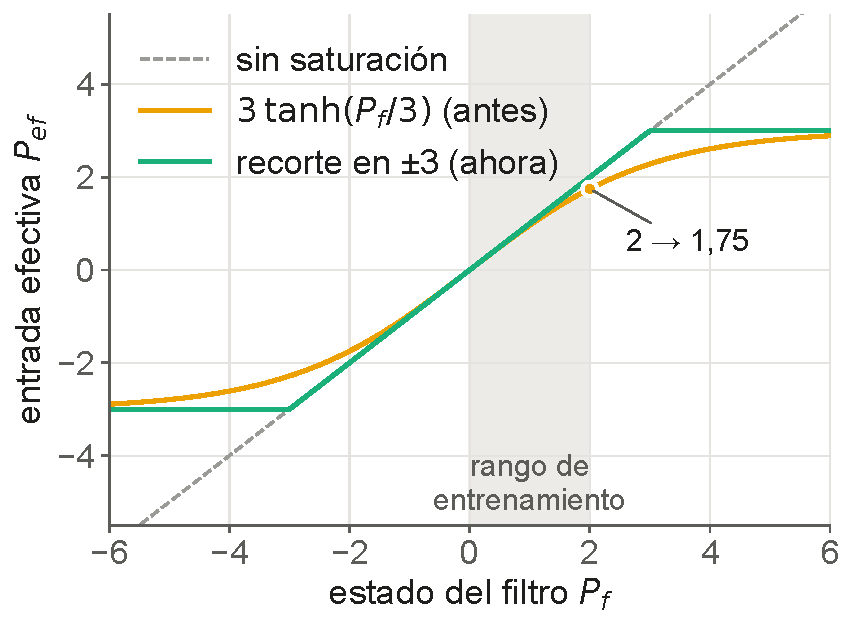
\includegraphics[width=0.6\textwidth]{saturacion.pdf}
\caption{Entrada efectiva $P_{ef}$ en función del estado del filtro $P_f$ para la saturación anterior y el recorte actual. La franja gris es el rango de comandos de los datos de entrenamiento.}
\end{figure}

La saturación con tanh comprime aun por debajo del nivel. Un comando de 2 sale como 1,75 y uno de 3 como 2,28. Esa compresión actúa dentro del rango de entrenamiento, así que el modelo la ve y la tiene que explicar con algo. El recorte es lineal hasta $\pm 3$ y deja como única perturbación el filtro, porque los comandos de entrenamiento no pasan de 2.

\begin{preguntas}
\pr{¿Por qué se cambió la tanh por el recorte?}
Porque la tanh agregaba una no linealidad dentro del rango de entrenamiento que no se buscaba estudiar. Los modelos la absorbían en $w_{EE}$, $w_{EI}$ y $a_e$, y el error de $\bh$ del estado de filtro quedaba entre 7 y 9 \% aun con poco ruido.

\pr{¿El recorte es más realista?}
Los dos son idealizaciones de la saturación de la opsina. El recorte se eligió para separar el efecto del filtro del efecto de la saturación. La línea con tanh se conserva como comparación.

\pr{¿Por qué los comandos de entrenamiento llegan solo a 2?}
Es el rango de los estímulos del dataset, que se diseñó antes del controlador. En lazo cerrado el controlador pide hasta $\pm 11$, y por eso el lazo cerrado mide también extrapolación.
\end{preguntas}

\section{Lazo abierto con tanh y con recorte}

\begin{figure}[H]
\centering
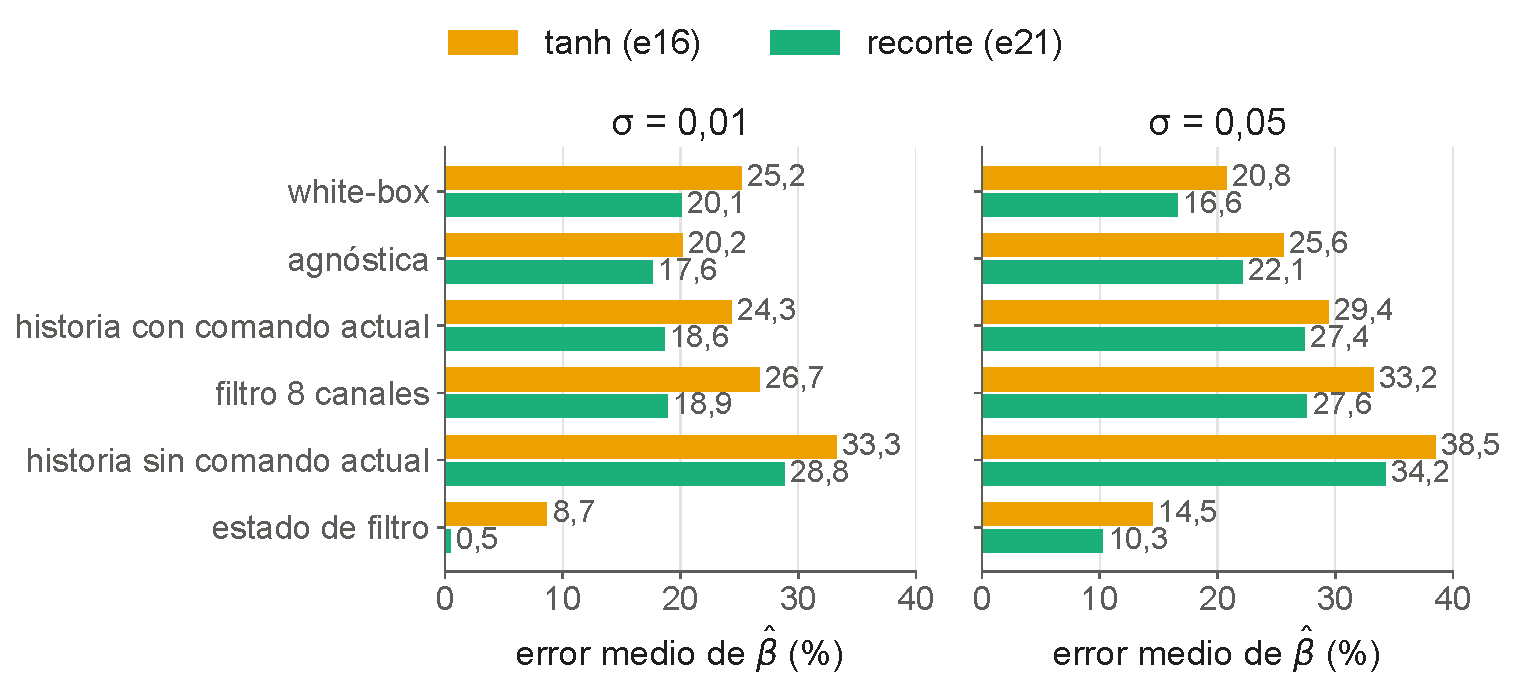
\includegraphics[width=\textwidth]{beta_tanh_vs_recorte.pdf}
\caption{Error medio de los diez parámetros, simulador con actuador, con tanh (e16) y con recorte (e21). Correcciones con red con warm start desde el white-box. La agnóstica con tanh tiene una sola semilla.}
\end{figure}

\begin{figure}[H]
\centering
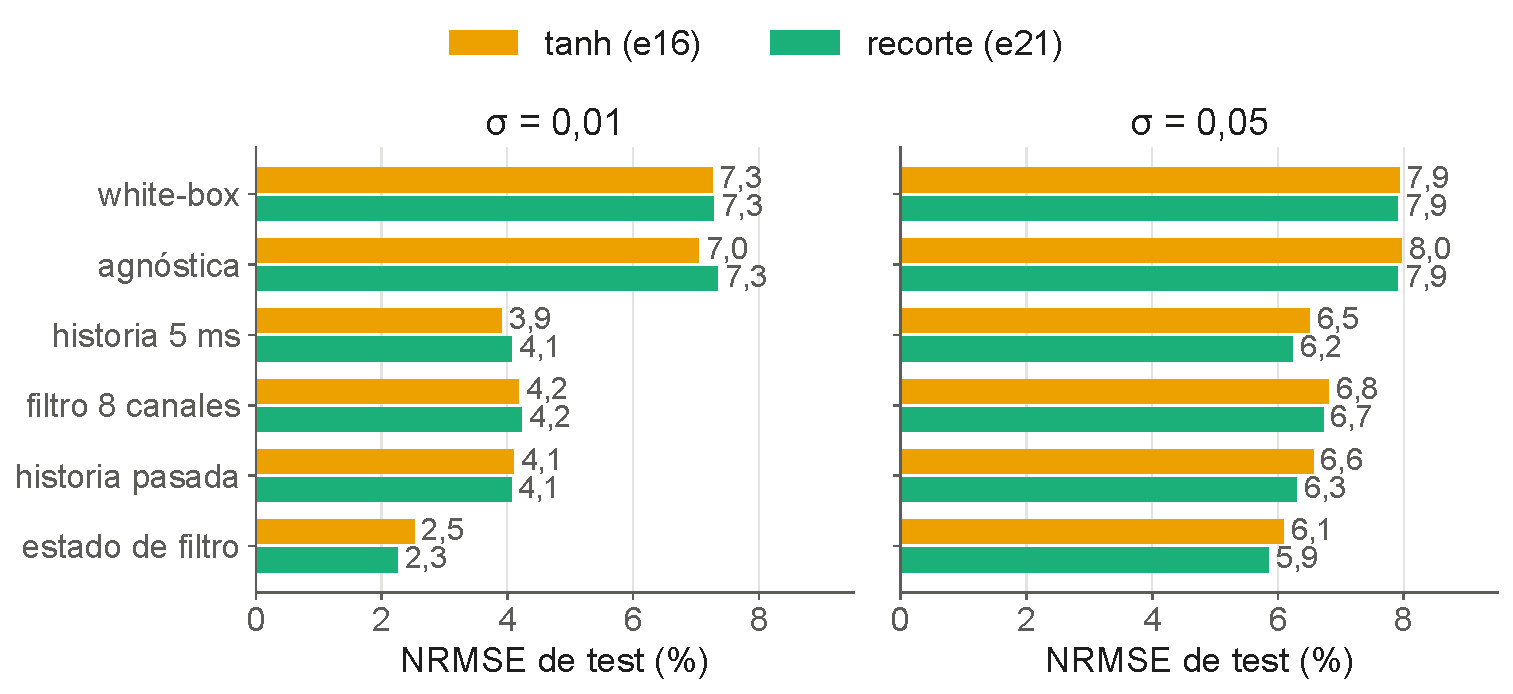
\includegraphics[width=\textwidth]{nrmse_tanh_vs_recorte.pdf}
\caption{NRMSE de test de los mismos modelos.}
\end{figure}

El recorte cambia poco la precisión en lazo abierto y cambia mucho la identificación. Con $\sigma = 0{,}01$ el estado de filtro pasa de 8,7 a 0,5 \% de error de $\bh$, con $\hat\tau = 0{,}997$~ms. Las correcciones con red mejoran algo, pero quedan entre 17 y 34 \%, porque su estructura no tiene el estado del filtro.

\begin{preguntas}
\pr{Si el NRMSE es parecido, ¿por qué importa el error de $\bh$?}
Porque dos modelos pueden reproducir igual de bien los datos con parámetros distintos. Si los parámetros están corridos, el modelo compensa con la red algo que debería explicar la física, y eso se nota al usarlo fuera de las condiciones de entrenamiento, como en lazo cerrado.

\pr{¿Por qué la agnóstica no mejora sobre el white-box en el actuador?}
Porque ve solo el estado $(I, E)$. El término faltante del actuador depende de la historia del comando, que la red no recibe.

\pr{¿Qué es el warm start?}
La corrección arranca con $\bh$ del white-box ya entrenado, en lugar de arrancar desde los valores iniciales. Cada configuración se corre también desde cero.
\end{preguntas}

\section{Capacidad de cada red con $\beta$ verdadero fijo}

\begin{figure}[H]
\centering
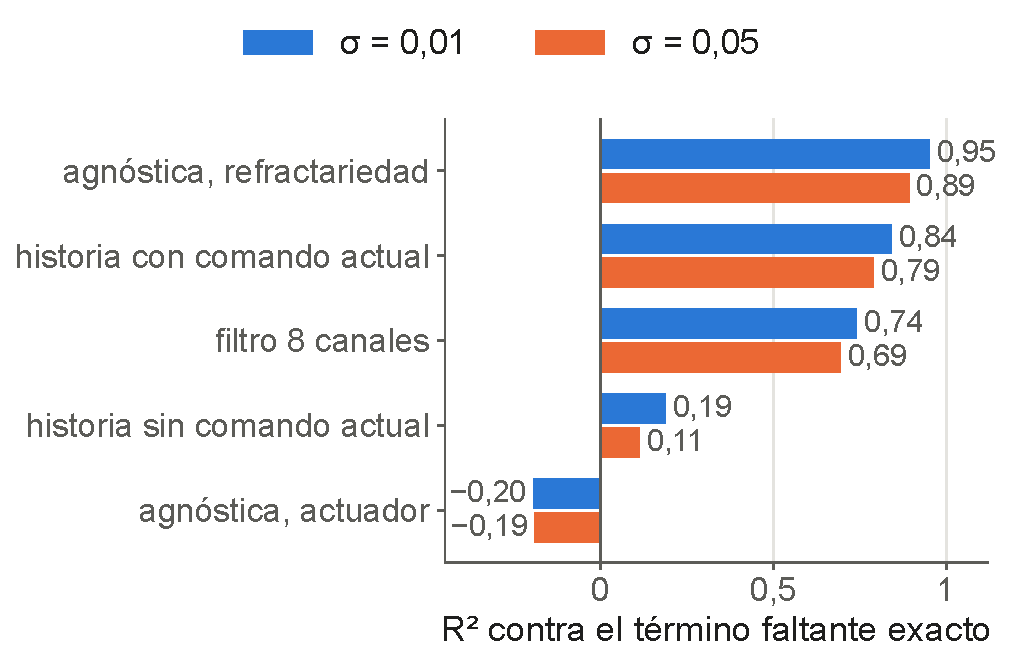
\includegraphics[width=0.65\textwidth]{beta_verdadero_r2.pdf}
\caption{R² de la red contra el término faltante exacto, con $\beta$ fijo en el valor verdadero y solo la red entrenable (e20). Primera fila, simulador refractario. Las demás, simulador con actuador con tanh.}
\end{figure}

Con $\beta$ fijo, la red no puede compensar con los parámetros, y el R² mide solo cuánto del término faltante puede representar. La historia con comando actual llega a 0,84 y la historia sin comando actual a 0,19. La diferencia viene del comando actual. El filtro de primer orden responde al comando en el mismo instante, y sin $u_k$ la red no puede reconstruirlo.

\begin{preguntas}
\pr{Si la historia sin comando actual representa tan poco, ¿por qué su NRMSE con $\beta$ libre es parecido al de la historia con comando actual?}
Porque con $\beta$ libre los parámetros absorben parte del término faltante. Su R² con $\beta$ libre es negativo ($-0{,}73$), y su error de $\bh$ es el más alto de las correcciones con red.

\pr{¿Por qué entonces se mantiene la historia sin comando actual?}
Porque es la única corrección con memoria del comando que deja el modelo explícito en $u_k$, y el controlador podría invertirla en forma cerrada (sección 2.3). En este paper se evalúa solo como planta.
\end{preguntas}

\section{x0 entrenable}

En el entrenamiento cada trayectoria se corta en ventanas de 5~ms, y cada ventana arranca desde el estado medido. Con ruido, ese estado inicial tiene error, y el error entra como condición inicial exacta. La segunda etapa arranca del modelo ya entrenado y deja entrenable el estado inicial de cada ventana, con un término que pide continuidad entre ventanas consecutivas. En el estado de filtro se liberan solo los estados iniciales de $E$ e $I$. El del filtro sale de filtrar el comando, que se conoce sin ruido.

\begin{figure}[H]
\centering
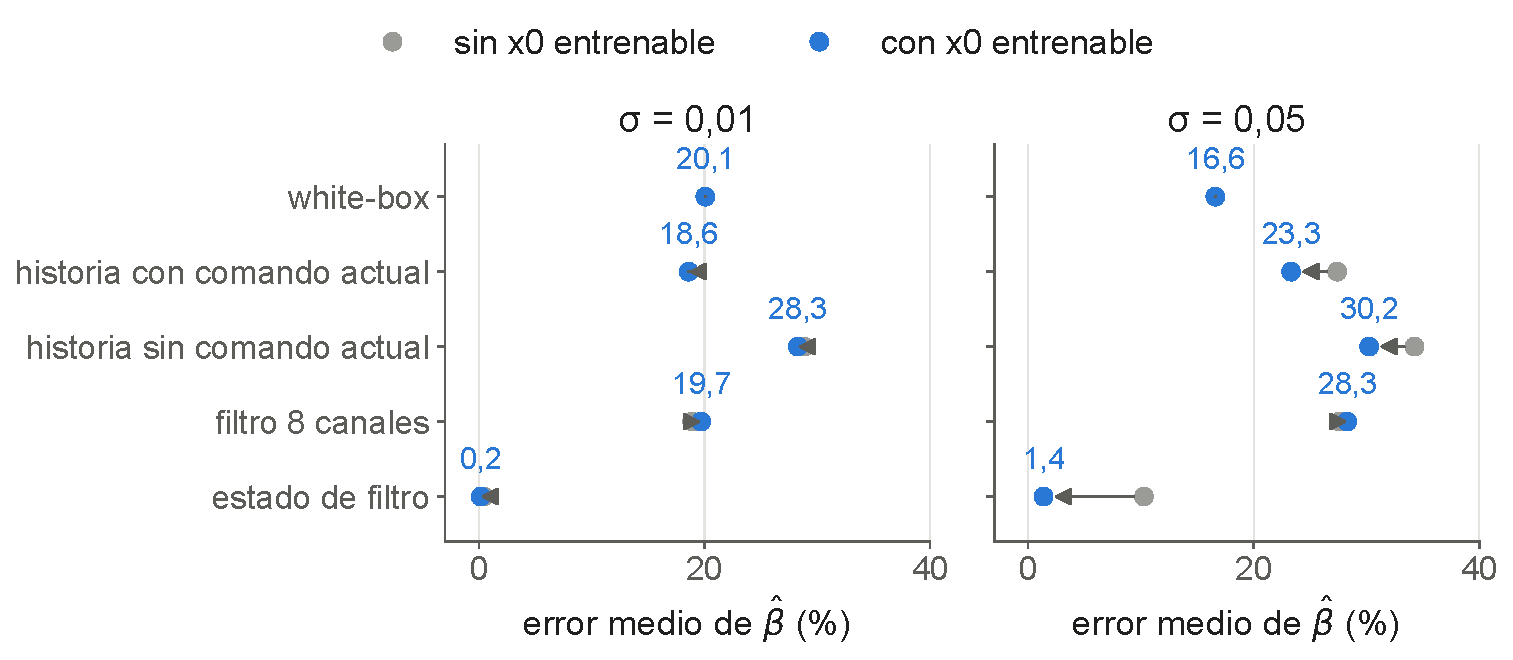
\includegraphics[width=\textwidth]{x0_entrenable_beta.pdf}
\caption{Error de $\bh$ antes (gris) y después (azul) de la segunda etapa. Correcciones con red en e22, estado de filtro en e23, desde el checkpoint de e21. El modelo de partida compite en la selección por validación.}
\end{figure}

\begin{preguntas}
\pr{¿Por qué x0 entrenable baja tanto el error en el estado de filtro y casi nada en las redes?}
Porque el error de $\bh$ tiene dos fuentes. El ruido en las condiciones iniciales sesga los parámetros, y x0 entrenable lo corrige. En el estado de filtro con $\sigma = 0{,}05$ el error baja de 10,3 a 1,4 \%. En las redes la fuente principal es estructural, porque les falta el estado del filtro, y liberar x0 no lo resuelve.

\pr{¿Por qué con $\sigma = 0{,}01$ casi no cambia nada?}
Con poco ruido el sesgo por condiciones iniciales es chico. El estado de filtro ya tenía 0,5 \% y baja a 0,2 \%.

\pr{¿Por qué en una versión anterior el white-box empeoraba de 20 a 35 \%?}
Era un artefacto de la selección del modelo. De cada entrenamiento se guarda la época con mejor validación, pero en la segunda etapa el modelo de partida no competía. En el white-box los x0 libres bajan la pérdida de entrenamiento absorbiendo el desajuste del modelo, y la validación empeora en todas las épocas. Se guardaba igual la mejor de esas épocas. Con el modelo de partida como candidato, el white-box queda en su valor original. El código ya está corregido.

\pr{¿x0 entrenable no permite que el modelo tape errores con las condiciones iniciales?}
Sí, si se usa desde el arranque. Por eso se aplica solo como segunda etapa, con el modelo ya entrenado, y con el término de continuidad. La selección por validación descarta el resultado si no mejora la reproducción de estímulos nuevos.
\end{preguntas}

\section{Lazo cerrado}

\subsection{Trazas}

\begin{figure}[H]
\centering
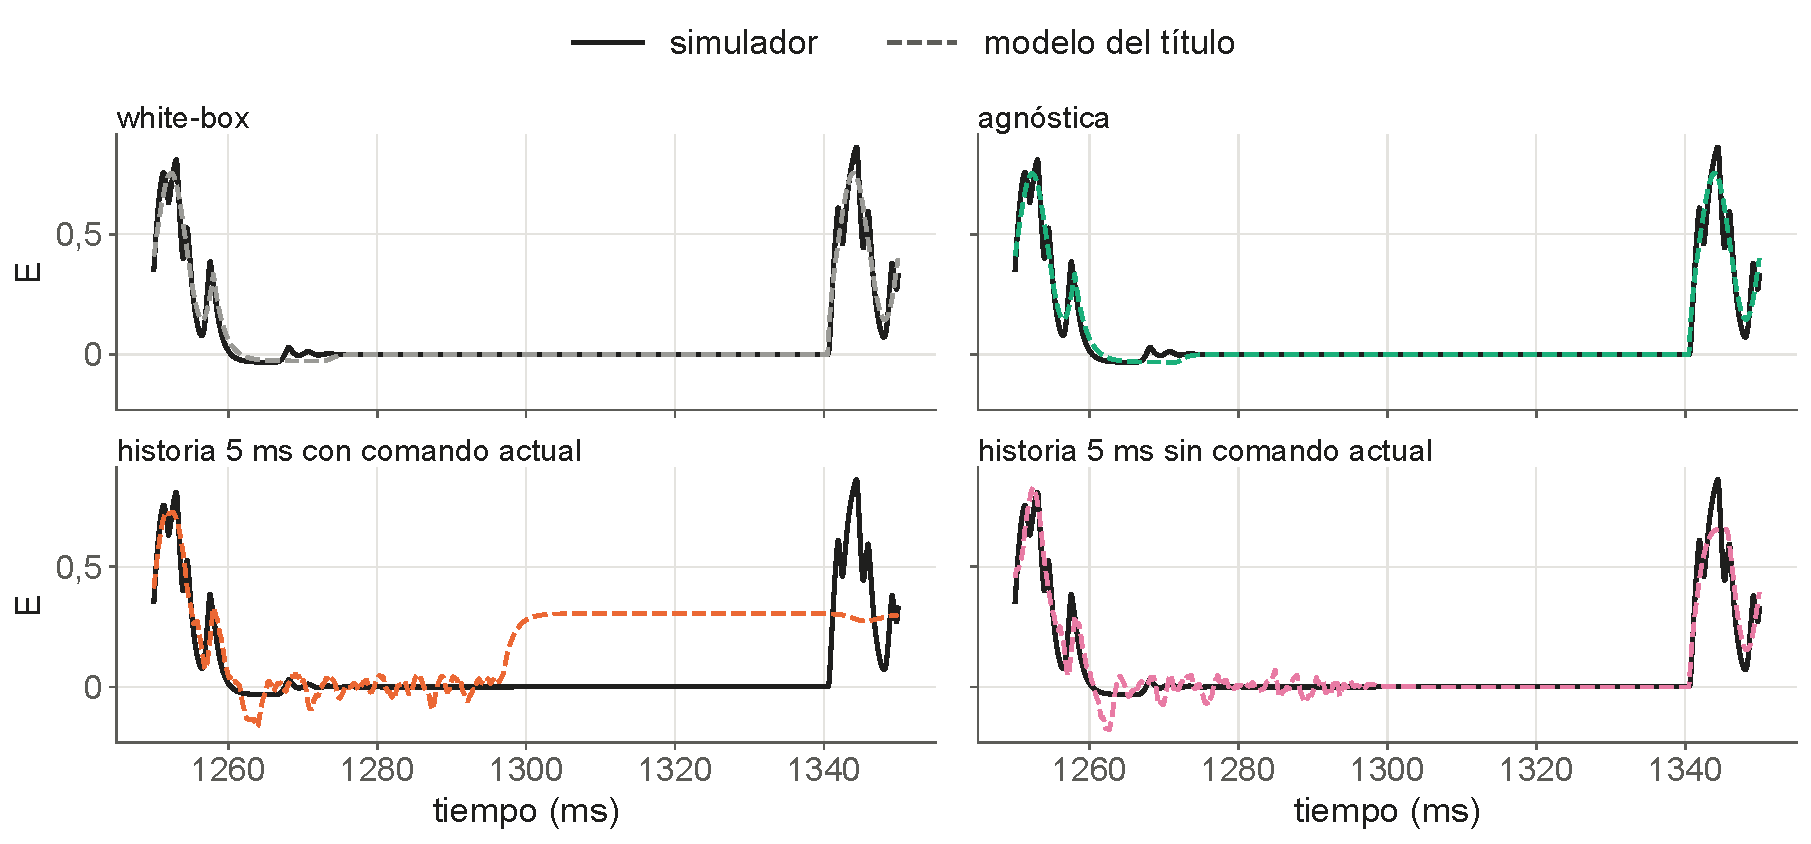
\includegraphics[width=\textwidth]{trazas_E_redes.pdf}
\caption{$E$ en lazo cerrado con el controlador del paper, referencia theta-gamma, entre 1250 y 1350~ms. En cada panel, el lazo con el simulador (continua) y el lazo con el modelo del título (discontinua). Modelos de la semilla 0 con $\sigma = 0{,}01$.}
\end{figure}

\begin{figure}[H]
\centering
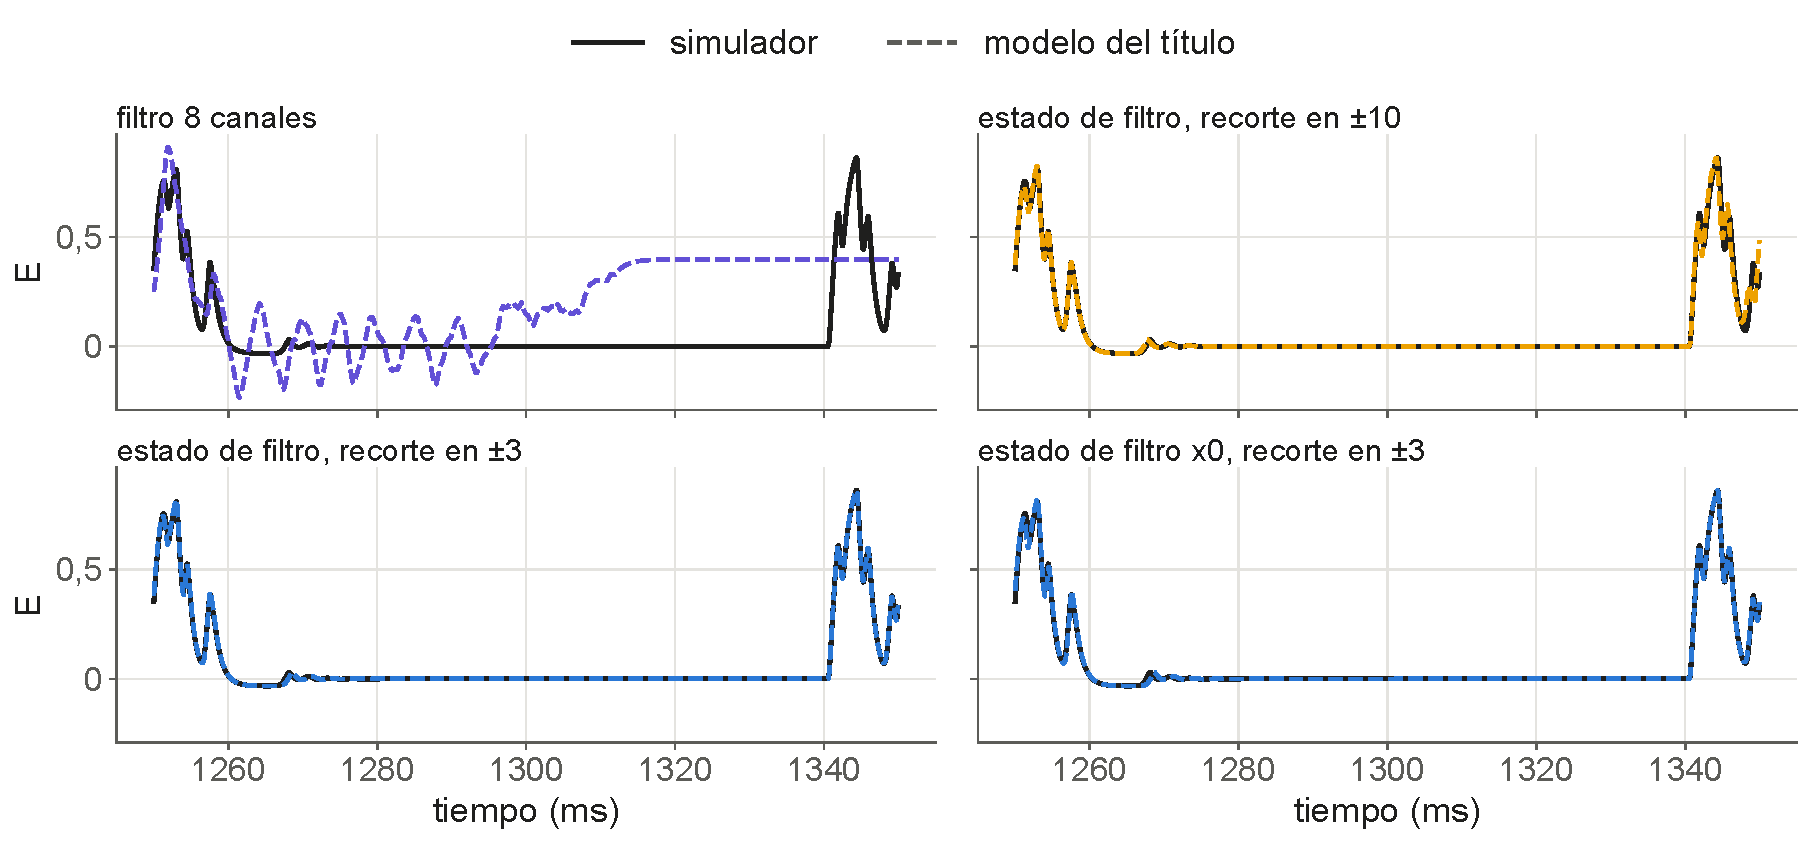
\includegraphics[width=\textwidth]{trazas_E_filtro.pdf}
\caption{$E$ en las mismas condiciones para el filtro de 8 canales y las tres versiones del estado de filtro.}
\end{figure}

\begin{figure}[H]
\centering
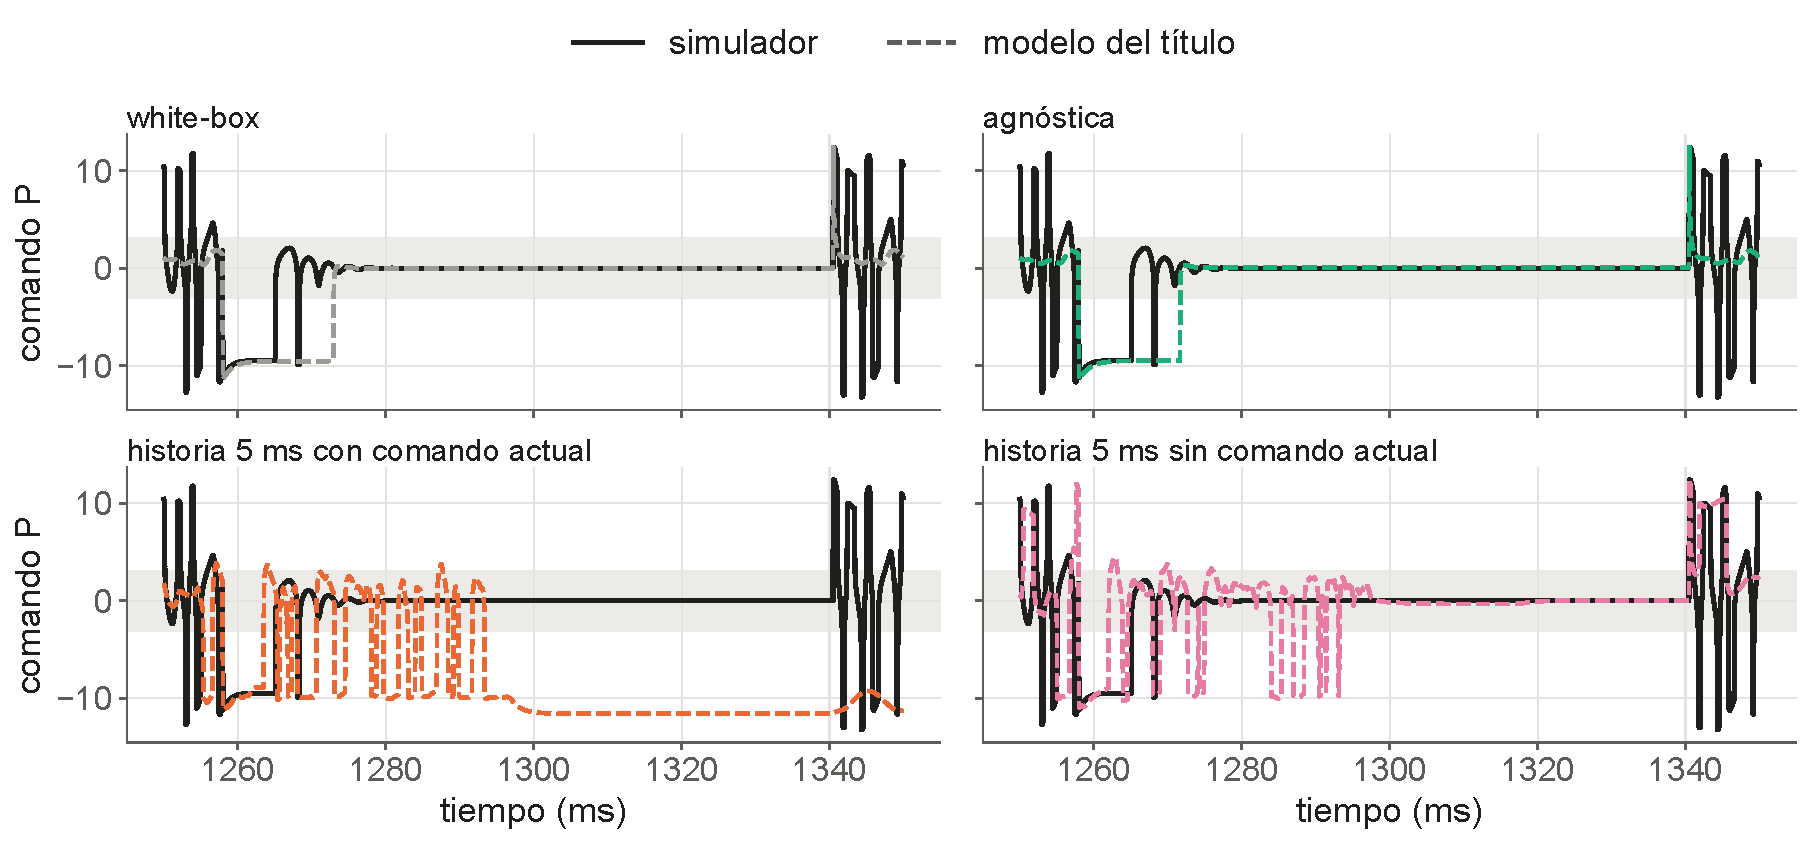
\includegraphics[width=\textwidth]{trazas_P_redes.pdf}
\caption{Comando $P$ que calcula el controlador en las corridas de la figura de $E$ con correcciones con red. La franja gris marca $\pm 3$, el nivel del recorte del simulador.}
\end{figure}

\begin{figure}[H]
\centering
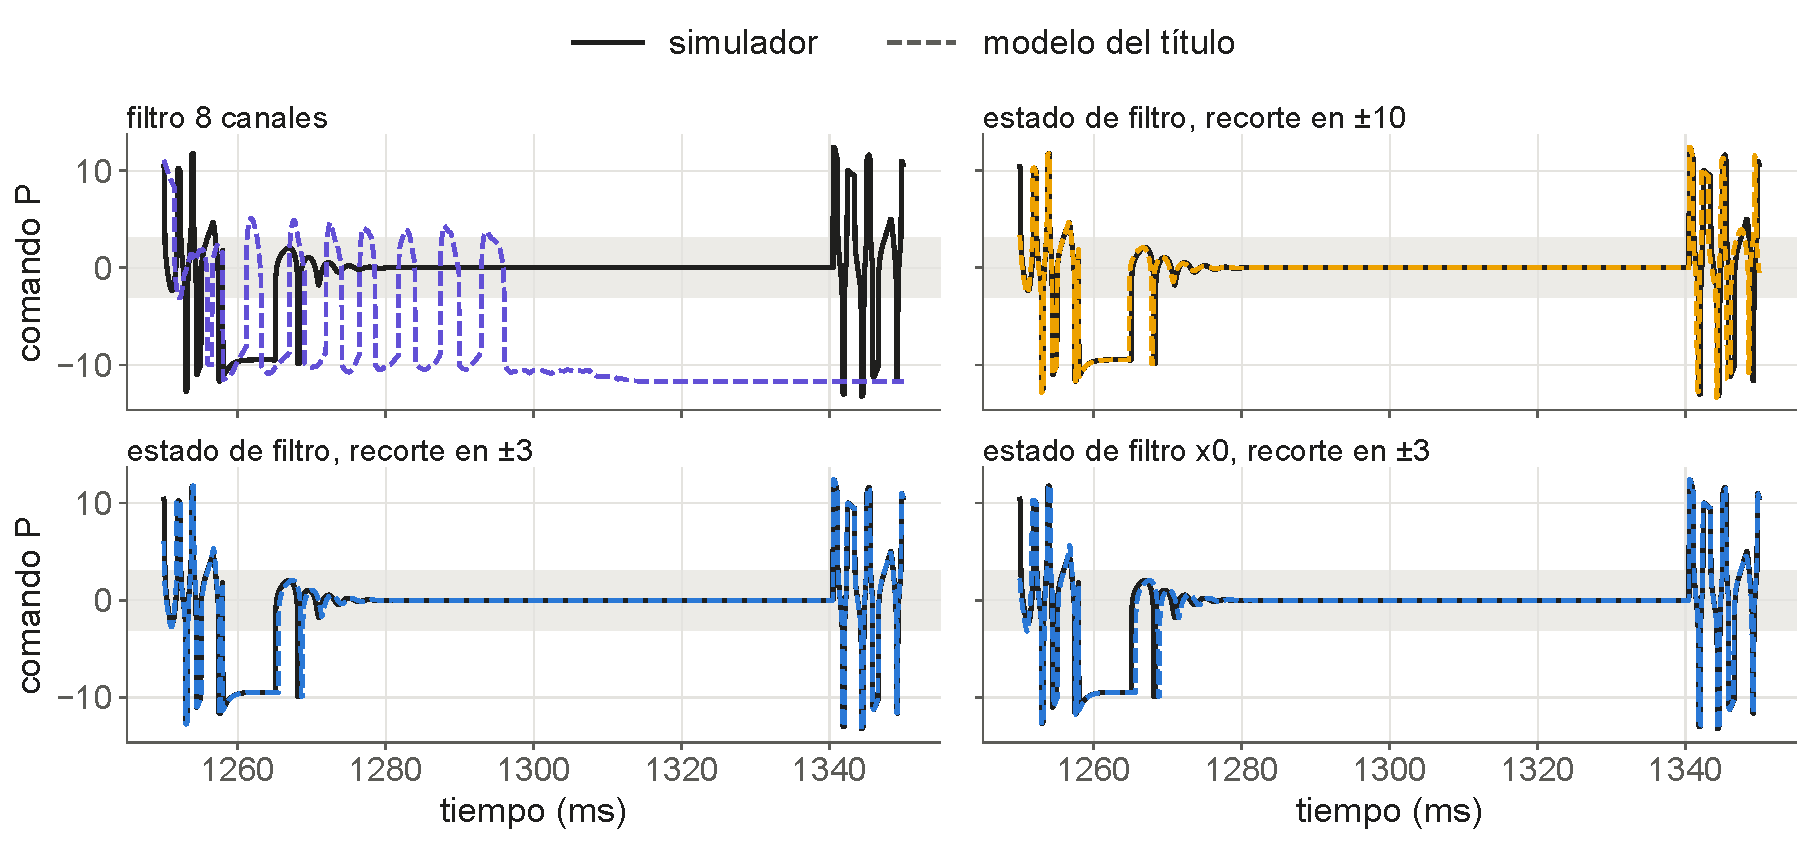
\includegraphics[width=\textwidth]{trazas_P_filtro.pdf}
\caption{Comando $P$ para el filtro de 8 canales y las tres versiones del estado de filtro.}
\end{figure}

Las trazas muestran tres comportamientos. El white-box y la agnóstica siguen el contorno de la actividad y suavizan los picos finos. Las correcciones con historia del comando oscilan entre los dos trenes de la referencia, donde el lazo con el simulador queda en reposo, y el controlador responde a esas oscilaciones con comandos de $\pm 10$. El estado de filtro con recorte en $\pm 3$ se superpone al simulador. Con recorte en $\pm 10$ se separa en los tramos donde el controlador pide más de 3, porque el modelo deja pasar lo que el simulador recorta.

\subsection{Distancia entre lazos}

Para comparar el lazo con un modelo y el lazo con el simulador se usa la distancia eficaz entre las dos trayectorias de $E$ e $I$, sobre el último 80 \% de la corrida, con $N$ muestras,
\[
d = \sqrt{\frac{1}{2N}\sum_{k}\Big[(E^{m}_k - E^{s}_k)^2 + (I^{m}_k - I^{s}_k)^2\Big]},
\]
con $m$ el lazo con el modelo y $s$ el lazo con el simulador. Es el criterio de identificación para control. Un modelo sirve si el lazo que se forma con él se parece al que se forma con la planta.

\begin{figure}[H]
\centering
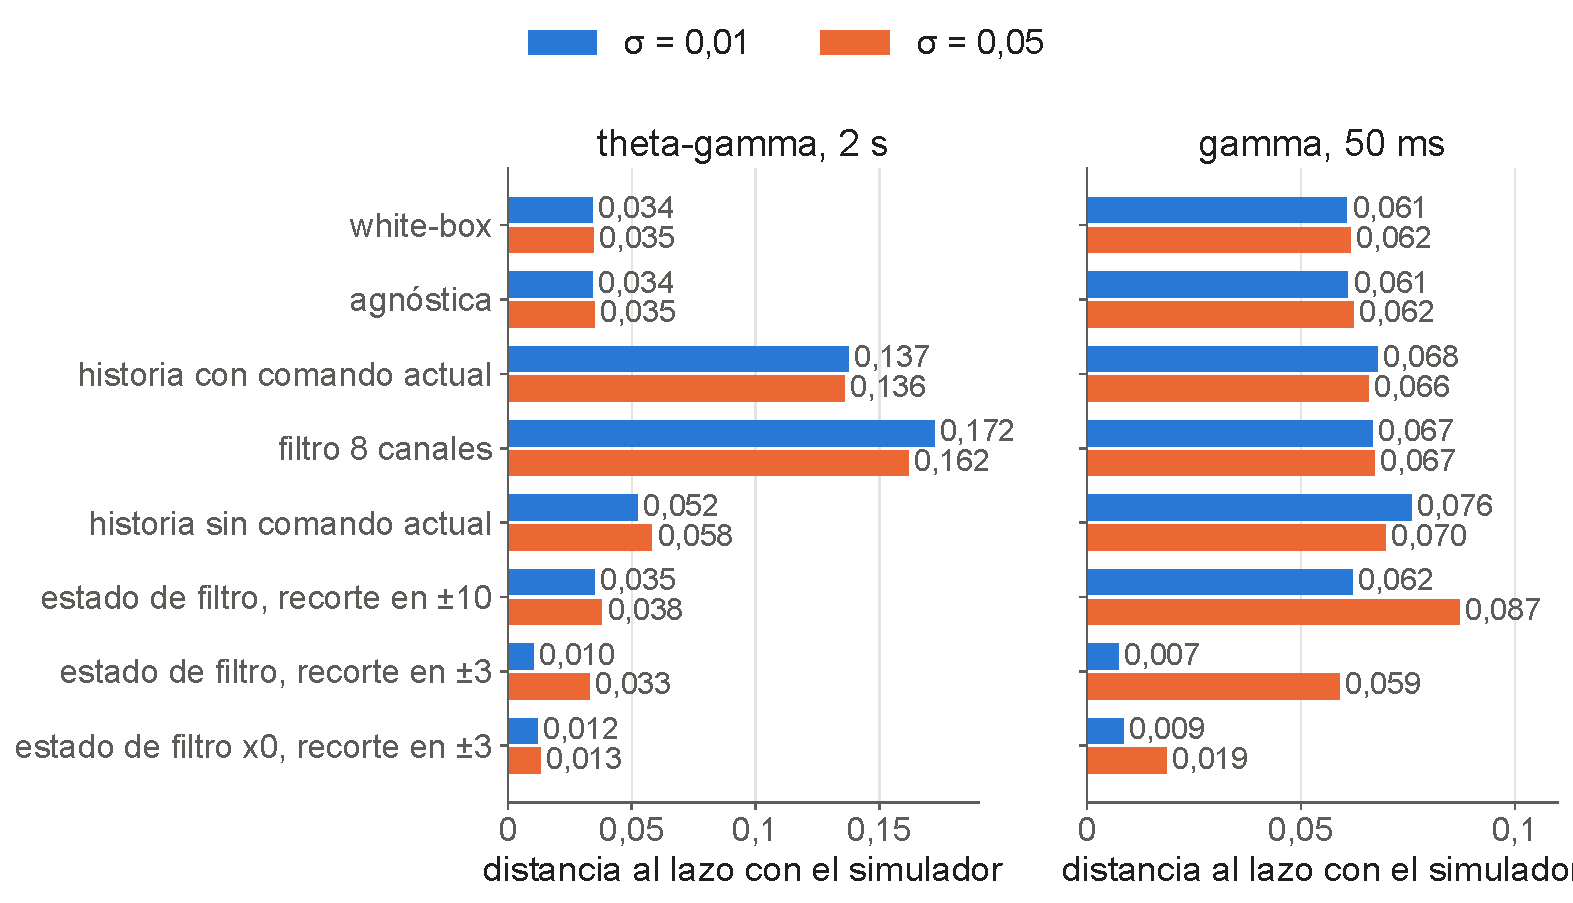
\includegraphics[width=\textwidth]{distancia_lazos.pdf}
\caption{Distancia al lazo con el simulador. Mediana de tres semillas, simulador con recorte.}
\end{figure}

\begin{figure}[H]
\centering
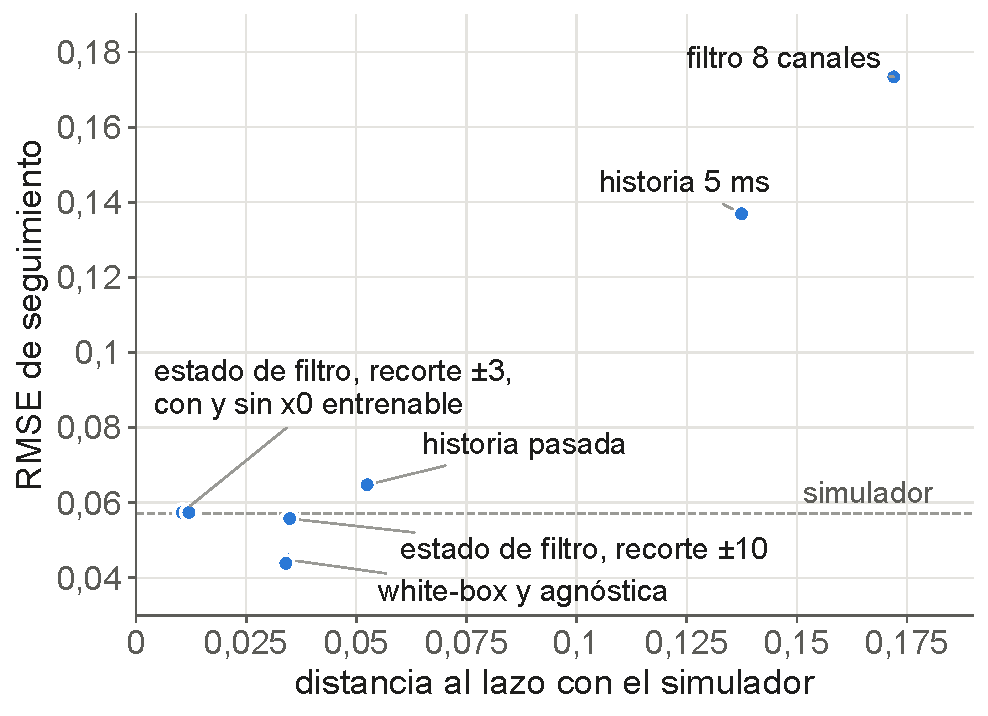
\includegraphics[width=0.62\textwidth]{rmse_vs_distancia.pdf}
\caption{RMSE de seguimiento contra distancia al lazo con el simulador, theta-gamma, $\sigma = 0{,}01$. La línea punteada es el RMSE del lazo con el simulador.}
\end{figure}

Con theta-gamma y $\sigma = 0{,}01$ el orden es claro. El estado de filtro con recorte en $\pm 3$ queda a 0,010, el white-box, la agnóstica y el estado de filtro con recorte en $\pm 10$ a 0,034 o 0,035, y las correcciones con historia entre 0,049 y 0,065. El RMSE de seguimiento no sigue ese orden. El white-box y la agnóstica siguen mejor que el simulador (0,045 contra 0,057), porque el controlador los cancela casi exactamente, y las correcciones con historia siguen casi como el simulador. Por eso el RMSE se reporta junto con la distancia.

Con gamma de 50~ms todos los modelos quedan entre 0,061 y 0,087, salvo el estado de filtro con recorte en $\pm 3$, que con $\sigma = 0{,}01$ queda en 0,007 sin x0 entrenable y en 0,009 con x0 entrenable.

\subsection{Nivel del recorte}

El nivel del recorte del estado de filtro no se identifica. Es un parámetro entrenable, pero el recorte solo recibe gradiente cuando el comando lo supera, y los comandos de entrenamiento no pasan de 2. El modelo se inicializa con el nivel en 10 y termina en 10. En la práctica es un valor fijado, igual que el 3 del diseño, que se le pone después sin reentrenar.

\begin{figure}[H]
\centering
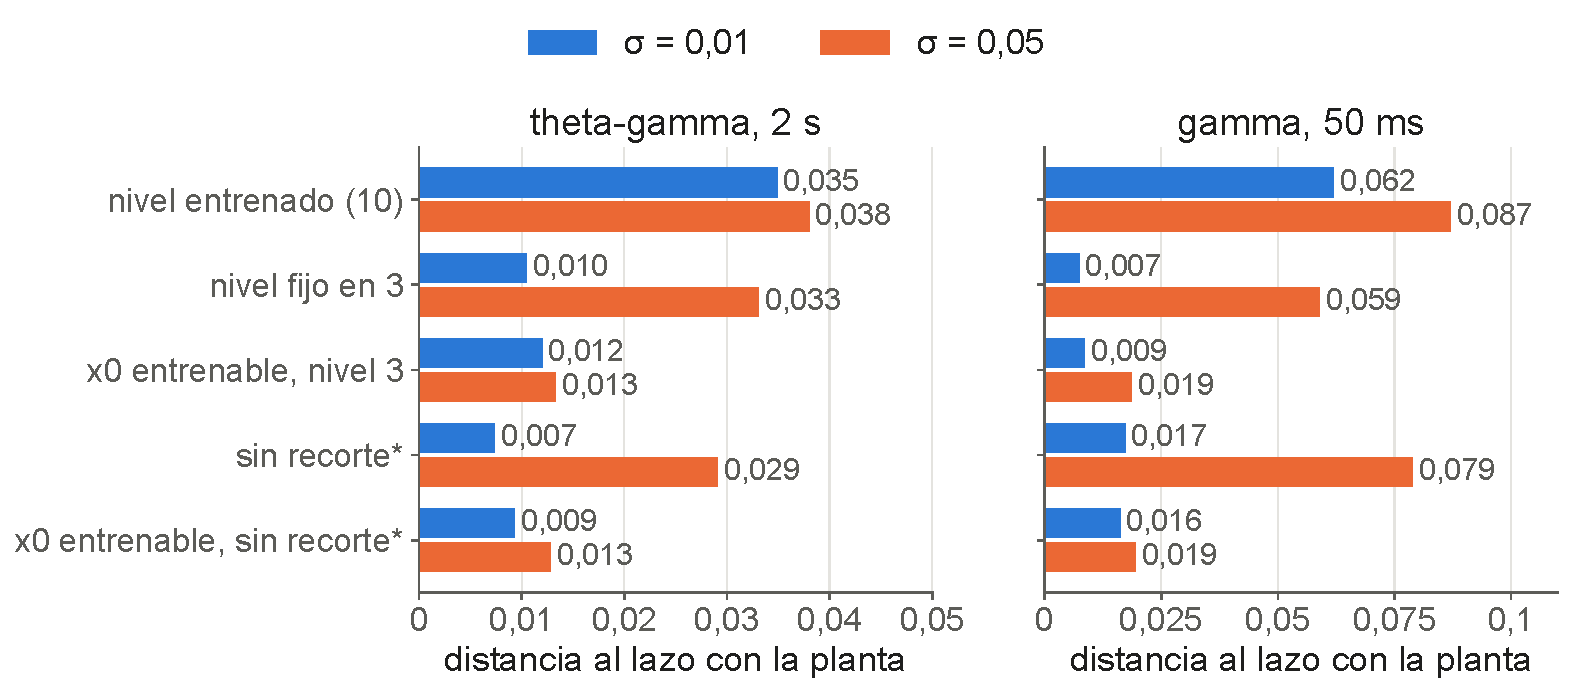
\includegraphics[width=\textwidth]{estado_filtro_en_lazo.pdf}
\caption{Distancia al lazo con el simulador para el estado de filtro. * Simulador con filtro y sin saturación, modelo sin recorte. Filas con x0 entrenable de e23, las demás de e21.}
\end{figure}

Con el recorte en $\pm 10$, el modelo deja pasar comandos de hasta 10 mientras el simulador los corta en 3, y el lazo se separa cada vez que el controlador pide más de 3. Con el recorte en $\pm 3$ y $\sigma = 0{,}01$ el lazo coincide. Con $\sigma = 0{,}05$ coincide recién con x0 entrenable, que corrige $\bh$. La distancia baja de 0,033 a 0,013 en theta-gamma y de 0,059 a 0,019 en gamma. Sin saturación en el simulador y sin recorte en el modelo pasa lo mismo.

\begin{preguntas}
\pr{¿Por qué el white-box sigue a la referencia mejor que el simulador?}
Porque el controlador invierte un Wilson-Cowan sin actuador, y el white-box tampoco tiene actuador. El controlador cancela el white-box casi exactamente y el seguimiento sale mejor que con el simulador, que sí tiene filtro y recorte. Por eso el seguimiento no sirve para elegir modelos y se reporta la distancia.

\pr{¿Se podría aprender el nivel del recorte?}
Con los datos actuales solo se puede acotar por abajo. Si se inicializa por debajo de 2, los comandos de entrenamiento lo superan, el gradiente lo empuja hacia arriba y se detiene cerca de 2. Un recorte en 2,01, en 3 o en 10 reproduce igual los datos. Para identificar el 3 hacen falta escenarios con comandos mayores a 3. Está anotado como corrida pendiente.

\pr{¿Fijar el nivel en 3 no es hacer trampa?}
El nivel de saturación del actuador es un dato del equipo de estimulación, que se conoce o se mide con un ensayo de comandos grandes. Fijarlo equivale a usar ese dato. Se reporta junto con el modelo que lo deja en su valor inicial.

\pr{¿Qué pasa con referencias que no sacan el comando del rango de entrenamiento?}
Con referencias theta de 8~Hz y gamma de 40~Hz construidas para eso, el estado de filtro reproduce el lazo del simulador con distancia menor a 0,001, y el white-box y la agnóstica quedan a menos de 0,003. Las diferencias grandes aparecen cuando el controlador pide comandos fuera del rango de entrenamiento.

\pr{¿Por qué en una versión anterior la historia con comando actual quedaba trabada en un valor fijo?}
Era un error de la simulación del lazo, corregido. El tiempo de la simulación se acumula sumando el paso de 0,005~ms, y el redondeo crece con la corrida. Desde los 1292~ms, el código que guarda el comando aplicado dejaba de reconocer el comienzo de cada paso y no lo guardaba más. La red veía el comando actual y una historia en cero, y con esa entrada el modelo tiene un punto fijo en $E = 0{,}243$, $P = -10{,}46$, donde quedaba el lazo. La historia sin comando actual no se trababa porque el comando actual entra solo por el backbone, que responde a un comando negativo bajando $E$. Se corrigió la tolerancia y se rehicieron todas las corridas afectadas, que eran las de theta-gamma con modelos con historia.

\pr{¿Por qué las correcciones con historia quedan más lejos que el white-box, si reproducen mejor en lazo abierto?}
Porque en lazo cerrado el controlador pide comandos entre $-13$ y $13$, y esas redes se entrenaron con comandos entre 0 y 2. Fuera de ese rango la red extrapola, y en las trazas aparecen oscilaciones que el simulador no tiene. El white-box no tiene una red que extrapole.
\end{preguntas}

\section{Referencia black-box}

\begin{figure}[H]
\centering
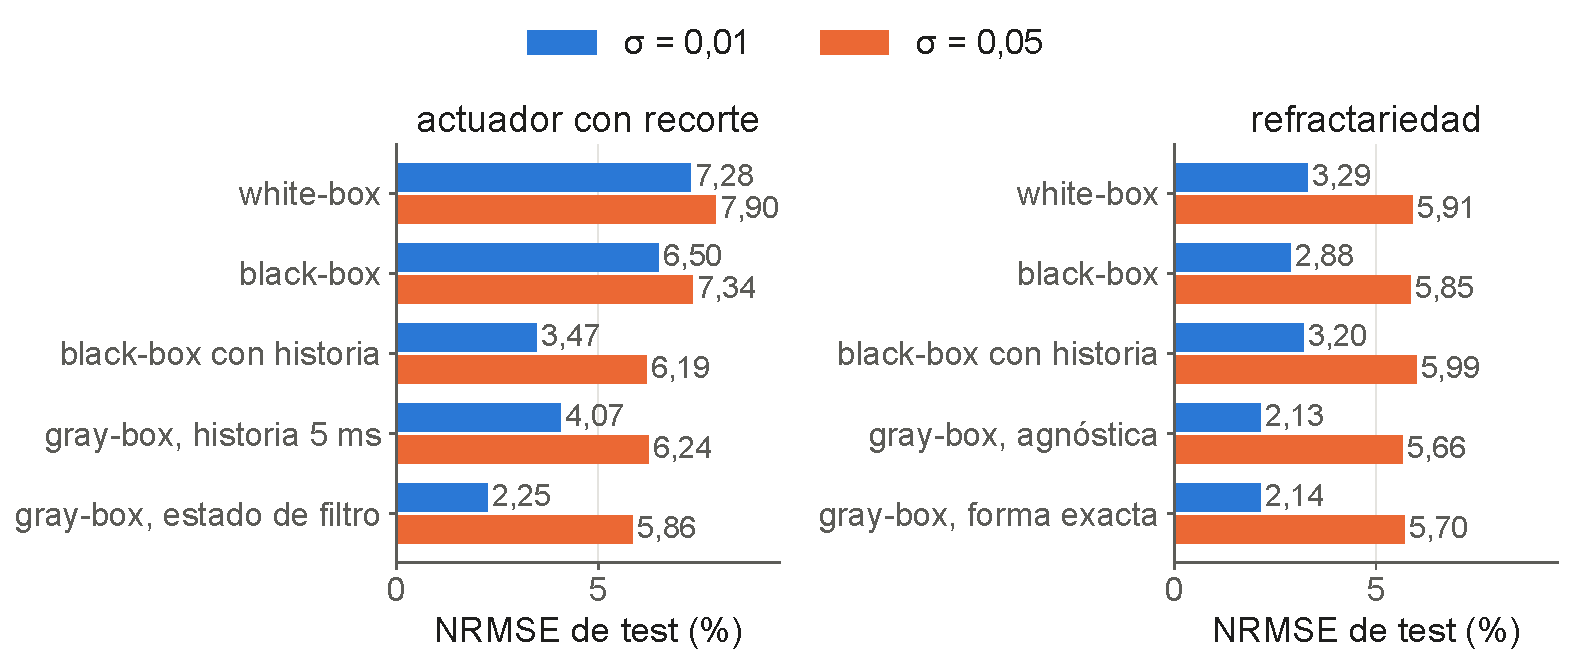
\includegraphics[width=\textwidth]{black_box.pdf}
\caption{NRMSE de test de la Neural ODE black-box $\dot x = g(I, E, P, Q)$ y de la misma red con historia del comando de 5~ms, con el white-box como referencia sin corrección y dos gray-box por perturbación. Red de 64 unidades, 3000 épocas, entrenada desde cero (e24).}
\end{figure}

La black-box sin historia mejora algo sobre el white-box en las dos plantas (6,50 contra 7,28 en el actuador y 2,88 contra 3,29 en la refractaria, con $\sigma = 0{,}01$). Con historia del comando, en el actuador supera a la corrección con red equivalente (3,47 contra 4,07 con $\sigma = 0{,}01$) y queda detrás del estado de filtro (2,25). En la refractaria queda detrás de la agnóstica y de la forma exacta.

\begin{preguntas}
\pr{Si la black-box con historia iguala a la corrección con red, ¿qué aporta el gray-box?}
Tres cosas. Los parámetros de Wilson-Cowan identificados, que la black-box no tiene. Las formas estructuradas, que son las más precisas en las dos plantas. Y, en las formas que no ponen el comando actual dentro de la red, la posibilidad de invertir el modelo en forma explícita dentro de un controlador (sección 2.3).

\pr{¿Por qué la black-box tiene una red más grande y más épocas?}
Porque aprende el campo vectorial entero y no una corrección chica sobre el backbone. Con la misma red que las correcciones quedaría en desventaja y la comparación no sería justa.

\pr{¿Por qué no se entrenó con warm start?}
Porque no hay backbone desde el cual arrancar. Es la única excepción a la regla de correr cada configuración con warm start y desde cero, y se declara en Métodos.

\pr{¿Se evaluó la black-box en lazo cerrado?}
Todavía no. Hace falta adaptar la simulación del lazo a un modelo sin backbone. Está pendiente.
\end{preguntas}

\section{Síntesis}

\begin{itemize}[leftmargin=*,itemsep=0.4em]
\item Con el recorte el actuador no comprime los comandos de entrenamiento, y el estado de filtro identifica $\beta$ con 0,5 \% de error con $\sigma = 0{,}01$.
\item El error de $\bh$ tiene dos fuentes. El ruido en las condiciones iniciales se corrige con x0 entrenable. La falta del estado del filtro en las redes no se corrige con x0.
\item La precisión en lazo abierto no alcanza para elegir un modelo para control. La distancia entre lazos separa los modelos.
\item El nivel del recorte no se puede aprender con comandos de entrenamiento de 0 a 2. Fijándolo en su valor conocido y con x0 entrenable, el lazo con el modelo coincide con el lazo con el simulador con los dos niveles de ruido.
\item En lazo abierto la black-box con historia iguala a la corrección con red. La ventaja del gray-box está en los parámetros identificables, en las formas estructuradas y en la inversión explícita.
\end{itemize}

\end{document}
